
\section {Methodology}
\label{sec:description}

%...................................................................................................................................................................................................

\subsection{Calculation of single $\mu$-like and single e-like ring p.d.f.s}
\label{sec:pdf_calculation}

{\color{red} 
Say a few general things about MC samples, and versions of software, flux and other tunes used. 
Or just cite specific sections of our past technotes and of the nue tech notes.

}

As stated in section \ref{sec:motivation}, the VaLOR joint oscillation analysis makes a simultaneous 3-flavour fit of the 
SuperK single $\mu$-like ring and single e-like ring spectra. The fit of the single $\mu$-like ring spectrum is made using 
the 3-flavour update of the official 2010 Rutherford-Oxford-Lancs Run 1+2 $\nu_{\mu}$-disappearance analysis described in 
\cite{OurRun1and2Analysis3F}. In this fit, the predicted single $\mu$-like ring spectrum is calculated using the same templates 
as in \cite{OurRun1and2Analysis3F}; these are $\nu_{\mu}$ CCQE, $\nu_{\mu}$ CC1$\pi$, $\nu_{\mu}$ CC other, $\nu_{\mu}$ NC, 
$\bar{\nu}_{\mu}$ CCQE, $\bar{\nu}_{\mu}$ CC1$\pi$, $\bar{\nu}_{\mu}$ CC other, $\bar{\nu}_{\mu}$ NC, background $\nu_{e}$ CCQE, 
background $\nu_{e}$ CC1$\pi$, background $\nu_{e}$ CC other, background $\nu_{e}$ NC, oscillated $\nu_{e}$ CCQE, oscillated 
$\nu_{e}$ CC1$\pi$ and oscillated $\nu_{e}$ CC other. 

In order to fit the number of single e-like ring events, a $\nu_{e}$-appearance analysis has also been developed in the same 
software framework. The predicted number of events is calculated using templates in {\color{red} give list of templates}.
This VaLOR $\nu_{e}$-appearance analysis is identical to the official 2010 analyses \cite{NueRun1Analysis, NueRun1and2Analysis} 
in all respects including event selection, flux tuning, systematic uncertainties and other inputs from the ND280 and SuperK. 
It was validated by comparing its results with those from the official $\nu_{e}$-appearance analyses, and this comparison is 
reported in Appendix \ref{app:standalone}.

Neutrino oscillation probabilities are calculated in a full 3-flavour framework including constant-density matter effects.
These calculations are made by custom software that has been developed in the VaLOR analysis framework. Details of this software,
its validation and estimates of its numerical accuracy are given in \cite{OurRun1and2Analysis3F}. A comparison between the
oscillation probabilities calculated by the VaLOR software and those given by Prob3++, which is used by many official T2K analyses,
is given in Appendix B in \cite{OurRun1and2and3Analysis3F}.

The passage of neutrinos through matter has a greater effect on the single e-like ring spectrum than on the single $\mu$-like
ring spectrum. In this technical note, the value of 3.2 g/cm$^{2}$ is used for the Earth density; this value is used \emph{so that 
the $\nu_{e}$-appearance part of the joint analysis can be validated by comparison with the 2010 official T2K $\nu_{e}$-appearance 
analyses \cite{NueRun1Analysis, NueRun1and2Analysis}, which use this value}. However in all future versions of the VaLOR joint
analysis, \emph{the value of 2.6 g/cm$^{2}$ will be used}.

%...................................................................................................................................................................................................

\subsection{Systematic parameters}
\label{sec:list_systematics}

This analysis considers systematic uncertainties from both the $\nu_{\mu}$-disappearance and the $\nu_{e}$-appearance analyses. 
These systematic uncertainties may be grouped into 3 categories:
\begin{itemize}
\item
Detectors 
\vspace{1.5 mm}

The uncertainties in the Super K 1R$\mu$ reconstruction efficiencies are taken from table 7.1 in \cite{TN065}. The uncertainties in the 
CCnonQE and NC efficiencies are energy-independent and are calculated by adding the corresponding seven components in that table in quadrature. 
The uncertainty in the CCQE efficiency is divided into the ring-counting and other efficiencies: the uncertainty in the ``other'' efficiency 
is calculated by adding CCQE components 1-3 and 5-7 in table 7.1 in \cite{TN065} in quadrature, and this is energy-independent. The uncertainty 
in the CCQE ring-counting efficiency is taken from equation 7.1 in \cite{TN065}; this is in the form of a covariance matrix in 3 bins of 
reconstructed energy (0-0.4, 0.4-1.1 and $>$1.1 GeV), and is propagated using the Cholesky method \cite{Cholesky}. 

The uncertainties in the Super K 1Re reconstruction efficiencies are taken from table 6 in \cite{NueRun1and2Analysis}. They are calculated 
by adding in quadrature the eight entries in that table for signal and background separately. 

The systematic uncertainty in the ND280 efficiency is calculated by adding in quadrature the $^{+4.2\%}_{-3.6\%}$ detector systematics and the 
3.7\% uncertainty related to the physics model \cite{ND280Error}.

\item
Flux
\vspace{1.5 mm}

The flux normalisation uncertainty was calculated using code provided by the beamline working group \cite{FluxNormError}. This 
uncertainty is expressed relative to the N$_{SK}$/N$_{ND280}$ ratio predicted by the MC, and is 4.7\% for nominal MC with oscillations 
with $\sin^{2}2\theta_{23}$ = 1.0 and $\Delta m^{2}_{32}$ = 2.32$\times$10$^{-3}$ eV$^{2}$/c$^{4}$. Without oscillations, this 
uncertainty is 7.3\%. The flux shape uncertainty was provided by the beamline working group as a covariance matrix in 19 bins of true 
energy \cite{FluxShapeError}.

\item
Cross sections
\vspace{1.5 mm}

The uncertainties in cross sections are taken from the presentation and ROOT file in \cite{NIWGErrors}. The uncertainty in the CCQE cross 
section represents the residual uncertainty that is not cancelled in the extrapolation from near to far detector; this residual 
uncertainty is due to the different flux energy ranges sampled by the near and far detectors and the different nuclear compositions of 
their targets. For this reason, it is applied only to the CCQE Super K templates. This uncertainty has a dependence on true energy, and this 
is taken from the ROOT file in \cite{NIWGErrors}.

The uncertainties in the other cross sections are expressed as a ratio to the CCQE cross section, and they are applied to the 
corresponding templates in both the ND280 and Super K. 

\end{itemize}

A complete list of these systematic uncertainties along with their numerical values is given in table \ref{tab:systematicslist}.


{\color{red} Need to add something about correlations between the two component analyses. }

\begin{table}[h]
\centering
\begin{tabular}{|c|c|c|c|c|c|}
\hline
 & & Systematic & Uncertainty & Applied to & Correlation\\
 & & parameter & & template(s) & between  \\
 & &  &  &  & 1R$\mu$ and 1Re \\
\hline
\hline
\multirow{16}{*}{Super K}  & \multirow{11}{*}{1R$\mu$ efficiencies} & CCQE ring counting & Covariance & $\nu_{\mu}$+$\bar{\nu}_{\mu}$ & \\
 &  & 3 E$_{reco}$ bins & matrix \cite{TN065} & CCQE (SK) & \\
 & & (correlated) &  &  & \\
\cline{3-6}
 & & CCQE other & 1.7\% \cite{TN065} & $\nu_{\mu}$+$\bar{\nu}_{\mu}$ & \\
 & &  &  & CCQE (SK) & \\
\cline{3-6}
 & & CCnonQE & 20\% \cite{TN065} & $\nu_{\mu}$+$\bar{\nu}_{\mu}$ CC1$\pi$ & \\
 & &  &  & + CCother (SK) & \\
\cline{3-6}
 & & NC & 111\% \cite{TN065} & $\nu_{\mu}$+$\bar{\nu}_{\mu}$ & \\
 & & &  \cite{TN065} & NC (SK) & \\
\cline{3-6}
 & & $\nu_{e}$ CC & 100\% & $\nu_{e}$ CC (SK) & \\
\cline{2-6}
 & \multirow{4}{*}{1Re efficiencies}& Signal & 7.6\% \cite{NueRun1and2Analysis} & All signal  & \\
 &  &  &  & $\nu_{e}$ (SK)  & \\
\cline{3-6}
 & & Background & 15\% \cite{NueRun1and2Analysis} & All background & \\
 &  &  &  & $\nu_{e}$ (SK)  & \\
\cline{2-6}
 &  & Energy scale & {\color{red} 2.3\% \cite{TN065} ?} & All SK &  \\
\hline
 ND280 & & Efficiency & +5.6\% -5.2\% \cite{ND280Error} & All ND280 & \\
\hline
\multirow{6}{*}{Flux} & & Normalisation & 4.7\% & & \\
 & & & (with oscillations, & & \\
 & & & using code in \cite{FluxNormError}) & & \\
\cline{3-6}
 & & Shape & Covariance & & \\
 & & 19 E$_{true}$ bins & matrix \cite{FluxShapeError} &  & \\
 & & (correlated) &  &  & \\ 
\hline
\multirow{21}{*}{Cross section} & \multirow{12}{*}{{\color{red}{1R$\mu$ + 1Re?}}} & CCQE & Depends on  & All CCQE (SK) & \\
 & & & true energy \cite{NIWGErrors} &  &  \\
\cline{3-6}
 & & CC1$\pi$/CCQE & 30\% (E$_{true}$$<$ 2 GeV) & All CC1$\pi$  &  \\
 & & & 20\% (E$_{true}$$>$ 2 GeV) & (SK and ND280)  &  \\
 & & & \cite{NIWGErrors} &  &  \\
\cline{3-6}
 & & CCcoh/CCQE & 100\% \cite{NIWGErrors}  & CC coherent  &  \\
  & & & & (SK and ND280) &  \\
\cline{3-6}
 & & CCother/CCQE & 30\% (E$_{true}$$<$ 2 GeV)  & All CCother  &  \\
 & & & 25\% (E$_{true}$$>$ 2 GeV)  & (SK and ND280) &  \\
 & & & \cite{NIWGErrors} &  &  \\
\cline{3-6}
 & & Nuclear effect & Depends on & {\color{red} All SK ?}&  \\
  & & {\color{red} is this FSI?} & reco energy {\color{red} (if FSI)} &  &  \\
\cline{2-6}
 & \multirow{2}{*}{{\color{red}{1R$\mu$ only?}}} & NC/CCQE & 36\% \cite{NIWGErrors} & All NC &  \\
 & & &  & (SK and ND280) &  \\
\cline{2-6}
  & \multirow{8}{*}{{\color{red}{1Re only?}}} & NC1$\pi^{0}$/CCQE & 30\% (E$_{true}$$<$ 1 GeV) & All NC1$\pi^{0}$ &  \\
  & & & 20\% (E$_{true}$$>$ 1 GeV) & (SK and ND280) &  \\
 & & & \cite{NIWGErrors} &  &  \\
\cline{3-6}
  & & NCcoh/CCQE & 30\% \cite{NIWGErrors} & All NC coherent &  \\
  & & & & (SK and ND280) &  \\
\cline{3-6}
  & & NCother/CCQE & 30\% \cite{NIWGErrors} & All NC other &  \\
  & & & & (SK and ND280) &  \\
\cline{3-6}
 & & $\nu_{e}$/$\nu_{\mu}$ & 6\% \cite{NIWGErrors} & All $\nu_{e}$ (SK) &  \\
\hline
\end{tabular}
\caption{Systematic parameters considered in the joint oscillation analysis 
{\color{red}Table not complete. Should there be a ND280 normalisation systematic ? Is the SK energy scale systematic 2.3\% for 1R$\mu$ 
(from \cite{TN065}) or 0.4\% (signal) and 1.1\% (background) for 1Re (from \cite{NueRun1and2Analysis}) or both ? }}
\label{tab:systematicslist}
\end{table}

\afterpage{\clearpage}

%...................................................................................................................................................................................................


\subsection{Neutrino oscillation fitting methodology}
\label{sec:fitter}

\subsubsection{Choice of oscillation parameters}
\label{sec:fitter:oscparams}

In this analysis, the mixing angles are used in the form $\sin^{2}\theta_{ij}$ and not $\sin^{2}2\theta_{ij}$. As mentioned in Sec.\ \ref{sec:motivation}, the leading-order 
term in P($\nu_{\mu} \rightarrow \nu_{e}$) depends on $\sin^{2}\theta_{23}$, and consequently it is natural to use $\theta_{23}$ in this form. Furthermore, it is not 
possible to distinguish the octant of $\theta_{23}$ when $\sin^{2}2\theta_{23}$ is used since both $\theta_{23}$ and $\pi/2 - \theta_{23}$ give the same value of 
$\sin^{2}2\theta_{23}$; this is clearly shown in Fig.\ \ref{fig:ambig}. By using the form $\sin^{2}\theta_{23}$, it might be possible to resolve this octant degeneracy. 

\begin{figure}[htbp]
\begin{center}
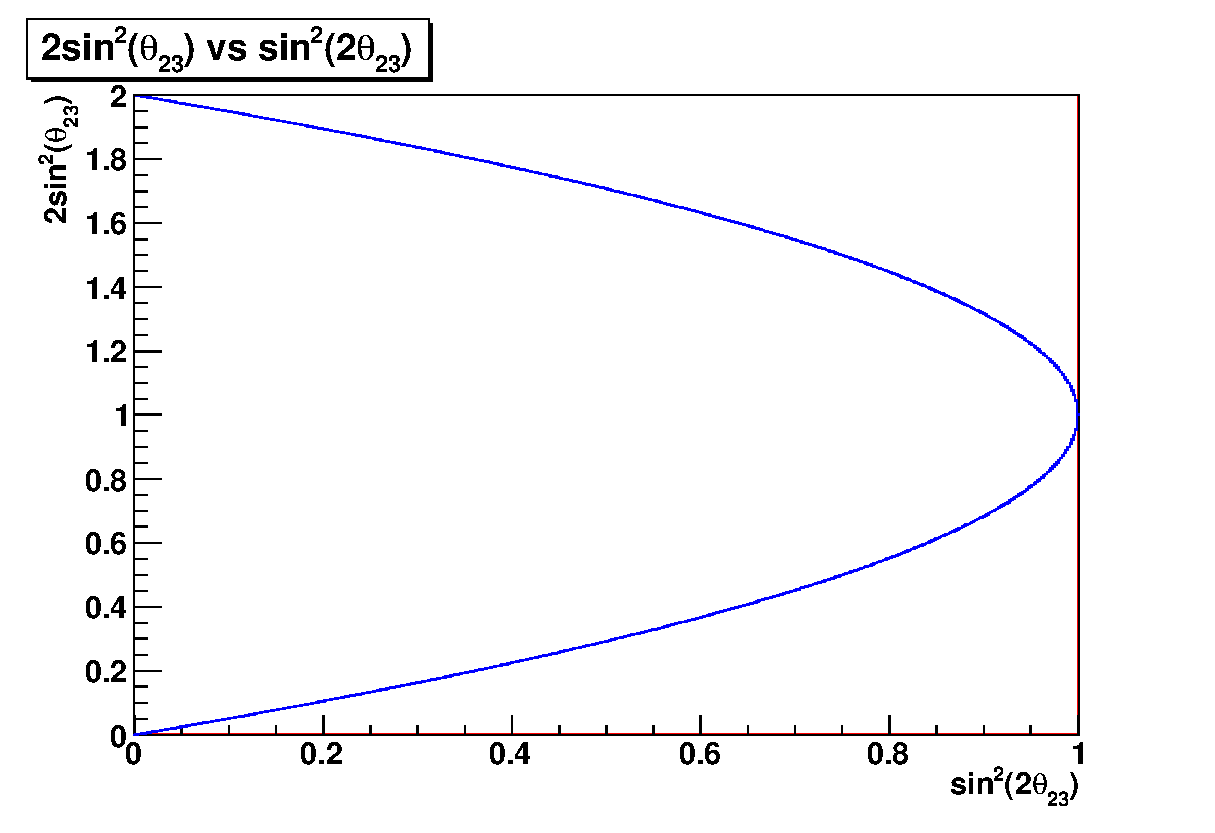
\includegraphics[width=0.5\textwidth]{images/description/Sin2thetaVsSin22theta.eps}
\caption{Values of $sin^{2}\theta_{23}$  vs $sin^{2}2\theta_{23}$. }
\label{fig:ambig}
\end{center}
\end{figure}

The use of $\sin^{2}\theta_{ij}$ also allows this joint oscillation analysis to be compared with global fits performed by theorists in  
\cite{LisiGlobalAnalysis} and \cite{ConchaMaltoniGlobalAnalysis}. In fact this is not the first time a neutrino oscillation 
experiment has used mixing angles in this form: for example, KamLAND has published results in terms of $\tan^{2}\theta_{12}$ \cite{KamLAND2008Paper}.

However the ability to use the form $\sin^{2}2\theta_{ij}$ has been retained, and this is used mainly for validating this joint analysis against the official T2K 
$\nu_{\mu}$-disappearance and $\nu_{e}$-appearance analyses. The VaLOR analysis framework allows straightforward and transparent switching between 
$\sin^{2}\theta_{ij}$ and $\sin^{2}2\theta_{ij}$ for the mixing angles. 

The mass-squared differences are input as $\Delta m_{21}^{2}$ and $|\Delta m_{32}^{2}|$. The mass hierarchy is set using the sign of $\Delta m_{32}^{2}$: 
this is positive for the normal hierarchy and negative for the inverted hierarchy. $\Delta m_{31}^{2}$ is not input but is calculated as $\Delta m_{31}^{2}$ 
= $\Delta m_{21}^{2}$ + $\Delta m_{32}^{2}$ for both hierarchies.

In this technical note, all results assume the normal mass hierarchy unless otherwise stated. 

The VaLOR group has also implemented a definition of the ``atmospheric'' mass-squared difference introduced by Fogli and Lisi \cite{Fogli}:
\begin{equation}
\Delta m_{FL}^{2} = m_{3}^{2} - \frac {m_{1}^{2}+m_{2}^{2}} {2}  =  \frac {\Delta m_{31}^{2} + \Delta m_{32}^{2}} {2} 
\end{equation} 
The quantity denoted $\Delta m_{FL}^{2}$ is useful since its absolute value is the same for both hierarchies, and only its sign changes. It helps to overcome the 
problem that $|\Delta m_{31}^{2}|$ is the largest mass-squared difference for the normal hierarchy whereas $|\Delta m_{32}^{2}|$ is the largest for the inverted 
hierarchy. The mass hierarchy is set using the sign of $\Delta m_{FL}^{2}$, and $\Delta m_{31}^{2}$ and $\Delta m_{32}^{2}$ are not input but are calculated from 
the input values of $\Delta m_{21}^{2}$ and $|\Delta m_{FL}^{2}|$. Again it is possible to switch the input of the mass-squared difference between $|\Delta m_{32}^{2}|$ 
and $|\Delta m_{FL}^{2}|$ in a straightforward and transparent way. 

$\Delta m_{21}^{2}$ and $|\Delta m_{FL}^{2}|$ will be used as inputs of the mass-squared differences in future versions of the joint oscillation analysis (though in 
this version $\Delta m_{21}^{2}$ and $|\Delta m_{32}^{2}|$ are used).

\subsubsection{Treatment of solar (12-sector) oscillation parameters}

A study has been made in which $\sin^{2}2\theta_{12}$ and $\Delta m_{21}^{2}$ were allowed to float in the fit of the single $\mu$-like ring Super K sample, and 
the results are shown in Appendix \ref{sec:solar}. It was found that the fitter returned extreme values of these parameters (see Fig.\ \ref{fig:solarfit}), and 
this is because they have no effect on the single $\mu$-like ring sample. For this reason, these parameters were fixed throughout this analysis to the values 
in table \ref{tab:solarparameters}.

\begin{table}[h]
\centering
\begin{tabular}{|c|c|}
\hline
Parameter & Value \\
\hline
\hline
$\sin^{2}2\theta_{12}$ & 0.87 \\
\hline 
$\Delta m_{21}^{2}$ & 7.6$\times$10$^{-5}$ eV$^{2}$/c$^{4}$ \\
\hline
\end{tabular}
\caption{Values used for $\sin^{2}2\theta_{12}$ and $\Delta m_{21}^{2}$ in the joint oscillation analysis}
\label{tab:solarparameters}
\end{table}

\subsubsection{Treatment of systematic parameters}

{\color{red} Blah blah blah}


\subsubsection{Initial values and allowed range of fit parameters}
\label{sec:initvalues_range}

{\color{red} Lorena, we shouldn't really constrain the systematic parameters in that narrow $\pm$1$\sigma$ range}

The initial values of the fit parameters and their allowed ranges are shown in Tab. \ref{tab:initvalues}. Wider limits for the systematic 
parameters were tried, but, since the fitter only rarely returned values $>$+1$\sigma$ or $<$-1$\sigma$, the limits were reduced to 
$\pm$1$\sigma$. When fitting toy experiments, the initial values of the fitted parameters are always different from the true input values 
in order to check that the fitter correctly recovers those input values.  
\begin{table}[h]
\centering
\begin{tabular}{|c|c|c|c|}
\hline
Parameter & Initial & Minimum & Maximum \\
\hline 
\hline
$|\Delta m_{32}^{2}|$ ($10^{-3} eV^{2}/c^{4})$ & 2.4  & 1.0 & 4.0\\
\hline
$\delta_{CP}$ & 0 &  -$\pi$ & +$\pi$ \\
\hline
$\sin^{2}2\theta_{23} $ & 0.9 & 0.6 & 1.0 \\
$\sin^{2}\theta_{23} $ (1$^{st}$ octant) & 0.4 & 0.2 & 0.6 \\
$\sin^{2}\theta_{23} $ (2$^{nd}$ octant) & 0.6 & 0.4 & 0.8 \\
\hline
$\sin^{2}2\theta_{13} $ & 0.09 & 0.0 & 0.42 \\
$\sin^{2}\theta_{13}   $ & 0.02 & 0.0 & 0.12 \\
\hline
Systematics & 0 & -??$\sigma$ &  +??$\sigma$ \\
\hline
\end{tabular}
\caption{Initial values and upper and lower limits for each oscillation parameter when fitted. The last row gives the nominal value 
         and upper and lower limits of systematic parameters when they are fitted.}
\label{tab:initvalues}
\end{table}
It was found that the fitter does recover the true input values of all parameters except $\sin^{2}\theta_{23}$. This parameter has two minima 
(one for each octant) as shown in Fig. \ref{fig:mirrordef}. There is a problem with fitting it since the fitter always returns a value in the 
same octant as the initial value irrespective of the true input value. For this reason, the fit is performed twice when $\sin^{2}\theta_{23}$ 
is one of the fitted parameters. In the first fit, $\sin^{2}\theta_{23}$ is given an initial value of 0.4 and a range of 0.2-0.6, while, in the 
second fit, it has an initial value of 0.6 and a range of 0.4-0.8. Subsequently the lowest value of -2 ln$\, \lambda$ in equation \ref{eq:chisqtot} 
from the two fits is chosen as the best fit. When making the two fits for $\sin^{2}\theta_{23}$, it is necessary to extend the allowed ranges 
up to 0.6 for the first octant fit and down to 0.4 for the second octant fit since the centre of symmetry between the two octants is $>$ 0.5 if 
$\theta_{13}$ is non-zero. This centre of symmetry is at 0.5 only if $\theta_{13}$ = 0 (this is shown in Appendix \ref{app:symmetry}).  

\begin{figure}[htbp]
\begin{center}
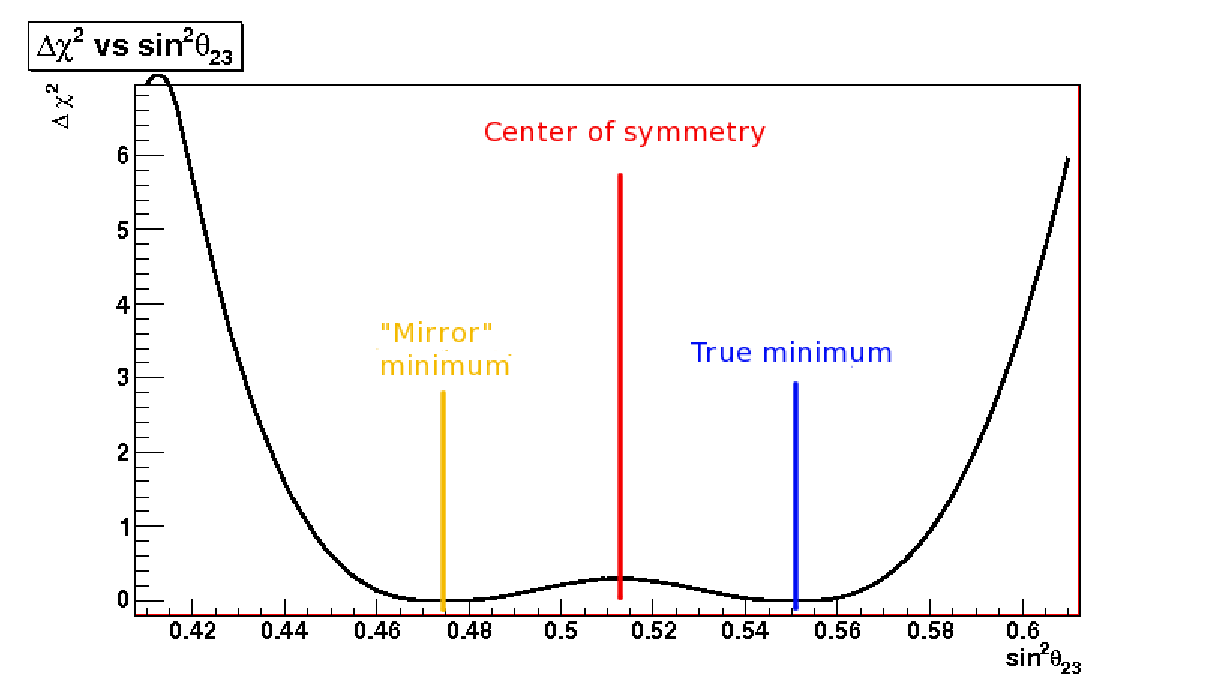
\includegraphics[width=0.8\textwidth]{images/description/GraphicalDefinitionOctants.eps}
\caption{Graphical definition of concepts true minimum, \textit{mirror} minimum and center of symmetry (assuming the true input value for  $sin^{2}\theta_{23}>0.5$).}
\label{fig:mirrordef}
\end{center}
\end{figure}


\subsubsection {Minimization method}

Measurements of the oscillation parameters are obtained by comparing the observed and predicted reconstructed one $\mu$-like ring energy spectra 
and the observed and expected numbers of one e-like ring events in Super K. A binned likelihood-ratio method is used for the one $\mu$-like ring 
sample and a counting experiment for the one e-like ring sample. Best-fit values of $\sin^{2}\theta_{23}$, $|\Delta m^{2}_{32}|$, $\sin^{2}\theta_{13}$ 
and $\delta_{CP}$ are obtained by varying them in the inputs to the calculation of the expected one $\mu$-like ring spectrum and the expected number 
of one e-like ring events until the following quantity is minimised:
\begin{equation}
\begin{split}
   -2 \, \ln{\lambda} 
    (\sin^{2}\theta_{23}, |\Delta m^{2}_{32}|, \sin^{2}\theta_{13}, \delta_{CP}; a)  
    &= 2 \displaystyle\sum_{i=0}^{N-1} \left[(n_{i,\mu-like}^{exp} - n_{i,\mu-like}^{obs}) 
    + n_{i,\mu-like}^{obs}ln\left(\frac{n_{i,\mu-like}^{obs}}{n_{i,\mu-like}^{exp}} \right)\right] \\
    &+ 2\left[ n_{e-like}^{exp} + ln(\Gamma (n_{e-like}^{obs} +1)) - n_{e-like}^{obs}ln(n_{e-like}^{exp}) \right] \\
    &+ (\boldsymbol{a} - \boldsymbol{a_{0}})^{T} C^{-1} (\boldsymbol{a} - \boldsymbol{a_{0}})
\end{split}
    \label{eq:chisqtot}
\end{equation}
In equation \ref{eq:chisqtot}, the first term is -2 $\times$ the log likelihood ratio for an observed number $n_{i,\mu-like}^{obs}$ and an expected 
number $n_{i,\mu-like}^{exp}$ ($\sin^{2}\theta_{23}$, $|\Delta m^{2}_{32}|$, $\sin^{2}\theta_{13}$, $\delta_{CP}$; {\bf a}) of one $\mu$-like 
ring events in the ith bin. {\color{red}{The sum is over 200 bins of reconstructed energy of width 50 MeV in the range 0-10 GeV - I have to update the binning... }}. 
This term is identical to the quantity that is minimised in the VaLOR $\nu_{\mu}$-disappearance analyses 
\cite{OurRun1DisappAnalysis2F, OurRun1and2Analysis2F, OurRun1and2Analysis3F, OurRun1and2and3Analysis3F} except that the expected energy spectrum 
depends on $\sin^{2}\theta_{13}$ and $\delta_{CP}$ as well as $\sin^{2}\theta_{23}$ and $|\Delta m^{2}_{32}|$. A full mathematical derivation of 
it is given in section 3.2 in \cite{OurRun1DisappAnalysis2F}. 
The second term is the -2 $\times$ the logarithm of a Poisson distribution with mean $n_{e-like}^{exp}$ and observed number $n_{e-like}^{obs}$, 
where $n_{e-like}^{obs}$ and $n_{e-like}^{exp}$ ($\sin^{2}\theta_{23}$, $|\Delta m^{2}_{32}|$, $\sin^{2}\theta_{13}$, $\delta_{CP}$; {\bf a}) 
are respectively the observed and expected numbers of one e-like ring events in Super K in a single reconstructed energy bin from 0-1.25 GeV. 
This term is identical to that used in the official T2K Run 1+2 $\nu_{e}$-appearance analyses \cite{NueRun1and2Analysis} except that the expected 
number of events depends on $\sin^{2}\theta_{23}$ and $|\Delta m^{2}_{32}|$ as well as $\sin^{2}\theta_{13}$ and $\delta_{CP}$. The third term is 
a penalty term for deviations of the systematic parameters from their nominal values; {\bf a$_{0}$} is a 1$\times$n$_{syst}$ vector of systematic 
parameters with nomimal values, where n$_{syst}$ is the number of systematics, {\bf a} is the same vector with fluctuated values, 
({\bf a} - {\bf a$_{0}$})$^{T}$ is the transpose of ({\bf a} - {\bf a$_{0}$}) and C is the systematic parameter covariance matrix of dimension 
n$_{syst}$$\times$n$_{syst}$. 

The notation -2 ln$\, \lambda$ is used interchangeably with $\chi^{2}$ for the quantity in equation \ref{eq:chisqtot} in this note. 

\subsubsection{Dealing with fitter failues}

{\color{red} What failure modes have you seen? What do you do if a fit fails? Do you re-run with different initial parameters?}


\subsubsection {Brief note on out fit labeling scheme}
\label{sec:oscfit_method_label}

{\color{red} The following scheme might simplify some of the text, especially the section where the joint analysis
is compared with stand-alone analyses and it always have to be clarified what parameters get fitted and on which samples.
If not, we can remove this section. Propose different labeling scheme if you want. }


In the following sections, the different fits are labeled as 
`$(F_{\theta12},F_{\theta13},F_{\theta23}+F_{{\Delta}m^2_{sol}},F_{{\Delta}m^2_{atm}}+F_{cp})$+$N_{syst}$', 
where
\begin{itemize}
\item
$F_{\theta12}$, $F_{\theta13}$ , $F_{\theta23}$ are boolean flags (0 or 1) indicating, respectively, whether the 12-, 13- and 23-sector
mixing parameters are allowed to float. As discussed in Sec. \ref{sec:fitter:oscparams}, the mixing parameters can be either
$\sin^{2}2\theta_{ij}$ or  $\sin^{2}\theta_{ij}$, depending on the chosen scheme, which will be clear from the context.
\item
$F_{{\Delta}m^2_{sol}}$, $F_{{\Delta}m^2_{atm}}$ are boolean flags indicating whether the solar and atmospheric squared mass splittings
are allowed to float. As discussed in Sec. \ref{sec:fitter:oscparams}, various schemes exist for these squared mass splittings.
A single scheme is used throughout this paper.
\item
$F_{cp}$ is a  boolean flag indicating whether the CP-invariance violating phase $\delta_{CP}$ is allowed to float in the fit.
\item
$N_{syst}$ represents the number of systematics parameters included in the fit.
If the symbol N is shown in place of $N_{syst}$, then all of the systematic parameters considered in the analysis are allowed to float.
If an actual number is shown, then it should be assumed that the chosen subset of systematic parameters includes the 
dominant ones.
\end{itemize}

Accoring to the above scheme, 
\begin{itemize}
\item
`(0,1,1+0,1+1)+N' is as fit of the 13- and 23-sector mixing angles, of ${\Delta}m^2_{32}$ and of $\delta_{CP}$. The 12-sector
mixing angle and ${\Delta}m^2_{21}$ are fixed. All systematics considered by the analysis are allowed to float.
\item
`(0,0,1+0,1+0)+5' is as fit of the 23-sector mixing angle and of  ${\Delta}m^2_{32}$. The value of ${\Delta}m^2_{21}$,
$\delta_{CP}$ and the other mixing angles are fixed. Only the 5 most important nuisance parameters are included in the fit.
\item
`(0,1,0+0,0+1)+0'  is as fit of the 13-sector  mixing angle and of $\delta_{CP}$. All other oscillation and systematic 
parameters are fixed.
\end{itemize}

%...................................................................................................................................................................................................

\subsection{Goodness-of-fit tests}

{\color{red} What is the statistic that tells us how good the fit was. See the 2012 disappearance paper.}

%...................................................................................................................................................................................................

\subsection{Systematic analysis}

{\color{red} Do you want to select 5-6 dominant systematics as was done in 2012 Run1+2+3 dissapearance?
This will simplify the fitter enormously. In view of the fact that there is some mistake in most plots and they have to be 
generated again, this is probably a very good idea. }

%...................................................................................................................................................................................................


\subsection{Toy-MC study of fitter performance}

{\color{red} Summarize results for the selected fitter (with the selected number of systematics). Point to appendices
for more details.}

%...................................................................................................................................................................................................

\subsection{Construction of confidence regions}

The preferred method of the VaLOR group for constructing confidence regions is the 
method of Feldman and Cousins \cite{FeldmanCousins} using, in presence of systematics, the Bayesian integration method
proposed by Cousins and Highland \cite{CousinsHighland}.
Indeed, this is the method employed in all our previous T2K oscillation analysis analyses 
\cite{OurRun1DisappAnalysis2F, OurRun1and2Analysis2F, OurRun1and2Analysis3F, OurRun1and2and3Analysis3F}.
However in this preliminary T2K joint 3-flavour oscillation analysis
we have used the simpler constant-$\Delta\chi^2$ method.
It is our intention to perform a full Feldman-Cousins construction when this analysis is repeated
on the Run 1+2+3 dataset using the latest (2012) analysis framework.

Let S be the set of oscillation parameters in which the $\chi^{2}$ surface is drawn, and
assume that N systematic parameters are allowed to float in the oscillation fit.
Let M be the set of oscillation parameters not included in S and not considered to be fixed
throughout the analysis.
The $\chi^{2}$ surface is constructed by calculating the $\chi^{2}$ values for a grid of points 
in the S parameter space. For each grid point, 
the parameters in S space are fixed to their true values
and the $\chi^{2}$ value is minimized with respect to the oscillation parameters in the M space and 
the N systematic parameters.
For example, when confidence regions are shown by the joint 3-flavour analysis in 
the ($\sin^{2}\theta_{23}$, $|\Delta m^{2}_{32}|$) space then, at each grid point in that space,
the value of $\chi^{2}$ has been minimised with respect to $\sin^{2}2\theta_{13}$, $\delta_{CP}$
and all N systematic parameters, while the solar oscillation parameters are fixed unless otherwise
stated.

When sensitivity studies are performed, the above procedure for the construction of a $\chi^{2}$ surface
is repeated for each toy MC experiment in an ensemble of $\sim10^3$ experiments with
randomized systematic parameters and including statistical fluctuations.

The allowed region of the oscillation parameter space is given by
\begin{equation}
\displaystyle
\chi^{2} < \chi_{min}^{2} + \Delta{\chi^{2}}_{critical}
\label{eq:chiconfregion}
\end{equation}
where $\chi_{min}^{2}$ is the minimum value of $\chi^{2}$ and the critical values of $\Delta{\chi^{2}}$ are 
2.30 (68\% CL), 4.61 (90\% CL), 5.99 (95\% CL), 9.21 (99\% CL) for 2 fitted parameters.

When drawing contours in the ($\sin^{2}\theta_{23}$, $|\Delta m^{2}_{32}|$) space, a {\em global} scan of the 
parameter space is used: a single best-fit point is found at the minimum value of $\chi^{2}$ in the whole 
parameter space, and the values of $\Delta{\chi^{2}}$ are calculated relative to it. However another method 
called a {\em raster} scan is used for drawing contours in the ($sin^{2}2\theta_{13}, \delta_{CP}$) space: 
for each value of $sin^{2}2\theta_{13}$, all the values of $\delta_{CP}$ from -$\pi$ to +$\pi$ are scanned, 
and the minimum value of $\chi^{2}$ is found for that value of $sin^{2}2\theta_{13}$. Then the values of 
$\Delta{\chi^{2}}$ are calculated relative to that minimum in order to find the allowed region for that value 
of $sin^{2}2\theta_{13}$. The difference between a global scan and a raster scan is that the former has a 
{\em single point} as best fit whereas the latter has a best-fit {\em line}. 

{\color{red} Don't really like the following:}
If, for an isolated point, the value of one of the best-fit oscillation parameters is dramatically different from the values of the same oscillation parameter in neighbouring points,
this point is considered a ``spurious'' one,  indicating a fitter failure. These points appear infrequently (less than 10 in a grid of 2000 points) and, in this work,
the value of $\chi^{2}$, obtained for these points by the fitter, is ignored and,  instead, it is interpolating from the neighbouring points.



 


